\chapter{Modeling with Compact Notation}

\begin{outcome}
\begin{itemize}
\item Review summation notation
\item Work on Sets, Parameters, Variables, and Model
\item Write compact formulations for linear programs
\end{itemize}
\end{outcome}

\begin{quote}
\itshape The models of the previous chapters fit on an index card: two or three variables, a handful of constraints, every coefficient written out by hand. Now imagine your client is a grocery chain: 40{,}000 products, 200 stores, 52 weeks of demand. Nobody---however patient---writes out that objective function term by term. And when next year's data arrive, nobody wants to retype the model. The notation of this chapter---sets, parameters, and summations---is how one page of mathematics describes a million-variable model, and how the same page describes it again next year when every number has changed.
\end{quote}

\section*{A Brief Review of Summation Notation and Its Relation to Vector Products}

Summation notation is a concise way to express the addition of a series of terms. It is commonly written as
\[
\sum_{i=m}^{n} \text{expression involving } i,
\]
where \(i\) is the index of summation, \(m\) is the starting index, and \(n\) is the ending index.

\underline{1. Sum of \(x_i\):}
\[
\sum_{i=1}^{n} x_i = x_1 + x_2 + \cdots + x_n.
\]
In vector terminology, if we let \(\mathbf{x}\) be an \(n\)-dimensional vector,
\[
\mathbf{x} = \begin{bmatrix} x_1 \\ x_2 \\ \vdots \\ x_n \end{bmatrix},
\]
then \(\sum_{i=1}^{n} x_i\) represents the sum of all components of \(\mathbf{x}\).

\underline{2. Sum of \(a_i x_i\):}
\[
\sum_{i=1}^{n} a_i x_i = a_1x_1 + a_2x_2 + \cdots + a_nx_n.
\]
This expression is the dot product (or inner product) of two \(n\)-dimensional vectors \(\mathbf{a}\) and \(\mathbf{x}\), where
\[
\mathbf{a} = \begin{pmatrix} a_1 \\ a_2 \\ \vdots \\ a_n \end{pmatrix}.
\]
In vector notation, the dot product is written as:
\[
\mathbf{a}^\top \mathbf{x} = \mathbf{a} \cdot \mathbf{x} = \sum_{i=1}^{n} a_i x_i.
\]
This product yields a scalar value that combines the corresponding components of the two vectors.

\section*{Notes on Sets, Indices, and Summation}

When modeling with compact notation, \emph{sets} help organize the problem and clearly indicate which indices appear in sums and constraints.

We typically denote sets with uppercase letters and use the corresponding lowercase letter as the index.  

\textbf{Example:}  
Let \( I \) be the set of months in the year:
\[
I = \{1, 2, 3, \dots, 12\}.
\]
We can write a sum over all months in two equivalent ways:
\[
\sum_{i \in I} a_i x_i \quad\text{or}\quad \sum_{i=1}^{12} a_i x_i.
\]

\medskip
\noindent
\textbf{Multiple Sets and Multiple Indices.}  
Sometimes, variables are indexed over \emph{two or more sets}.  
For example, let:
\[
J = \{\text{'red'}, \text{'green'}, \text{'blue'}\}
\]
and suppose we have a variable \( y_{ij} \) indexed by both \( i \in I \) (months) and \( j \in J \) (colors).

If, for each color \( j \), the sum of \( y_{ij} \) over all months must equal 1, we write:
\[
\sum_{i \in I} y_{ij} = 1 \quad \forall j \in J.
\]
This single compact expression actually represents \emph{three} constraints—one for each color—where in each case, 12 monthly variables are summed to equal 1.

\medskip
\noindent
\textbf{Important Rule: Every Index Must Be Defined.}  
In any mathematical expression, \emph{every index must appear either}:
\begin{enumerate}
    \item in a summation, or  
    \item in a ``for all'' (\(\forall\)) quantifier.
\end{enumerate}

In the above example, \( y_{ij} \) uses both indices \( i \) and \( j \).  
\begin{itemize}
    \item The summation \(\sum_{i \in I}\) defines \(i\).  
    \item The ``for all'' statement \(\forall j \in J\) defines \(j\).
\end{itemize}
Without these definitions, the mathematical meaning of the expression would be incomplete or ambiguous.

\begin{learningcheckpoint}[label={lc:missing-index}]
Consider the incorrect formulation:
\[
\sum_{i \in I} y_{ij} = 1
\]
Write down what is missing from this statement to make it mathematically complete. Which index is undefined, and how should it be introduced?
\end{learningcheckpoint}

\section{Production Planning Models}

\subsection*{Production Planning Model (for \(T\) Periods)}

\begin{center}
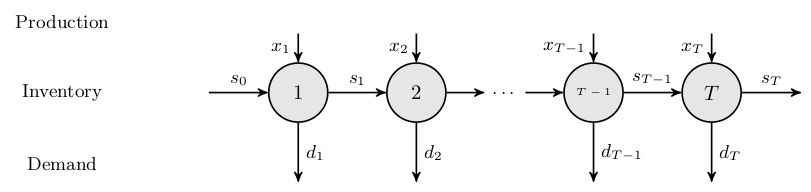
\includegraphics[width=0.85\linewidth]{figs/modeling-sums-tikz01.png}
\end{center}

\modelhead{Sets}
\begin{itemize}
    \item \(t \in \{1,2,\dots,T\}\): Periods in the planning horizon.
\end{itemize}

\modelhead{Parameters}
\begin{itemize}
    \item \(c^{prod}_t\): Production cost per unit in period \(t\) (for \(t=1,\dots,T\)).
    \item \(c^{inv}\): Inventory holding cost per unit carried from one period to the next.
    \item \(d_t\): Demand in period \(t\).
    \item \(s_0\): Initial inventory available at the start of period 1.
\end{itemize}

\modelhead{Variables}
\begin{itemize}
    \item \(x_t\): Number of units produced in period \(t\).
    \item \(s_t\): Inventory level at the end of period \(t\).
\end{itemize}

\modelhead{Model}
\begin{align*}
\min_{x,s} \quad & z = \sum_{t=1}^{T} \Big( c^{prod}_t\, x_t + c^{inv}\, s_t \Big)   \tag{Total cost} \\
\st        & s_0 + x_1 = d_1 + s_1   \tag{Period 1 balance} \\
                 & s_{t-1} + x_t = d_t + s_t &&\quad \text{for all } t=2,\dots,T   \tag{Inventory balance} \\
                 & x_t \geq 0,\quad s_t \geq 0 &&\quad \text{for all } t=1,\dots,T.
\end{align*}

\begin{examplewithallcode}{ Production Planning with 10 Periods (\(T = 10\))}
{https://github.com/open-optimization/open-optimization-or-book/blob/master/Intro-Math-Programming/baseText/optimization/optimization-examples/production-10period-excel.xlsx}
{https://github.com/open-optimization/open-optimization-or-book/tree/master/Intro-Math-Programming/baseText/optimization/optimization-examples/production_10period_pulp.ipynb}
{https://github.com/open-optimization/open-optimization-or-book/tree/master/Intro-Math-Programming/baseText/optimization/optimization-examples/production_10period_gurobi.ipynb}

\underline{Initial Inventory:}
\[
s_0 = 5 \quad \text{units}
\]

\modelhead{Data}
\href{https://github.com/open-optimization/open-optimization-or-book/blob/master/Intro-Math-Programming/baseText/optimization/optimization-examples/production-planning-data.xlsx}{(Download the data)}
\begin{center}
\begin{tabular}{@{}c*{10}{c}@{}}
\toprule
\textbf{Parameter}               & 1  & 2  & 3  & 4  & 5  & 6  & 7  & 8  & 9  & 10 \\ \midrule
Production Cost (\$ per unit)    & 10 & 12 & 14 & 16 & 18 & 20 & 22 & 24 & 26 & 28 \\
Demand (units)                   & 8  & 6  & 9  & 7  & 10 & 5  & 8  & 6  & 4  & 7  \\
\bottomrule
\end{tabular}
\end{center}

\underline{Inventory Holding Cost:}
\[
c^{inv} = 5 \quad \text{per unit}
\]

\modelhead{Variables}
\begin{itemize}
    \item \(x_t\): Number of units produced in period \(t\).
    \item \(s_t\): Inventory level at the end of period \(t\).
\end{itemize}

\modelhead{Model}
\begin{align*}
\min_{x,s} \quad & z = 10x_1 + 12x_2 + 14x_3 + 16x_4 + 18x_5 + 20x_6 + 22x_7 + 24x_8 + 26x_9 + 28x_{10} \\
                 & \quad + 5\,(s_1+s_2+s_3+s_4+s_5+s_6+s_7+s_8+s_9+s_{10})   \tag{Total cost} \\
\st        & 5 + x_1 = 8 + s_1   \tag{Period 1} \\
                 & s_1 + x_2 = 6 + s_2   \tag{Period 2} \\
                 & s_2 + x_3 = 9 + s_3   \tag{Period 3} \\
                 & s_3 + x_4 = 7 + s_4   \tag{Period 4} \\
                 & s_4 + x_5 = 10 + s_5   \tag{Period 5} \\
                 & s_5 + x_6 = 5 + s_6   \tag{Period 6} \\
                 & s_6 + x_7 = 8 + s_7   \tag{Period 7} \\
                 & s_7 + x_8 = 6 + s_8   \tag{Period 8} \\
                 & s_8 + x_9 = 4 + s_9   \tag{Period 9} \\
                 & s_9 + x_{10} = 7 + s_{10}   \tag{Period 10} \\
                 & x_t \geq 0,\quad s_t \geq 0 &&\quad \text{for all } t=1,\dots,10.
\end{align*}
\end{examplewithallcode}

\section*{Production Planning with Overtime}

A manufacturing firm seeks to optimize its production schedule over a \(T\)-day planning horizon to meet daily demand while minimizing costs. The firm starts with an initial inventory of \(s_0\) units. Production can be carried out during regular time and via overtime. The costs are as follows:
\begin{itemize}
    \item \textbf{Regular production cost:} \(c^{prod}_t\) dollars per unit on day \(t\).
    \item \textbf{Overtime production cost:} \(c^{over}_{t}\) dollars per unit on day \(t\).
    \item \textbf{Inventory cost:} \(c^{inv}\) dollars per unit carried over from one day to the next.
\end{itemize}

The goal is to determine the number of units to produce during regular time and overtime on each day, and the inventory levels, in order to minimize the total cost while satisfying daily demand.

\bigskip

\modelhead{Sets}
\begin{itemize}
    \item Days of production \( = \{1, 2, \dots, T\}\).
\end{itemize}

\modelhead{Parameters}
\begin{itemize}
    \item \(c^{prod}_t\): Regular production cost per unit on day \(t\) (for \(t=1,\dots,T\)).
    \item \(c^{over}_{t}\): Overtime production cost per unit on day \(t\) (for \(t=1,\dots,T\)).
    \item \(c^{inv}\): Inventory holding cost per unit carried to the next day.
    \item \(d_t\): Demand on day \(t\).
    \item \(s_0\): Initial inventory at the start of day 1.
\end{itemize}

\modelhead{Variables}
\begin{itemize}
    \item \(x_t\): Number of units produced in regular time on day \(t\).
    \item \(y_t\): Number of units produced in overtime on day \(t\).
    \item \(s_t\): Inventory at the end of day \(t\).
\end{itemize}

\modelhead{Model}
\begin{align*}
\min \quad & \sum_{t=1}^{T} \Big( c^{prod}_t x_t + c^{over}_{t} y_t + c^{inv} s_t \Big)   \tag{Total cost} \\
\st        & s_0 + x_1 + y_1 = d_1 + s_1   \tag{Day 1 balance} \\
             & s_{t-1} + x_t + y_t = d_t + s_t &&\quad \text{for all } t = 2,\dots,T   \tag{Inventory balance} \\
             & x_t,\, y_t,\, s_t \ge 0 &&\quad \text{for all } t = 1,\dots,T.
\end{align*}

\newpage

\begin{examplewithallcode}{Production Planning with Overtime (\(T = 10\))}
{https://github.com/open-optimization/open-optimization-or-book/blob/master/Intro-Math-Programming/baseText/optimization/optimization-examples/production-overtime-excel.xlsx}
{https://github.com/open-optimization/open-optimization-or-book/tree/master/Intro-Math-Programming/baseText/optimization/optimization-examples/production_overtime_pulp.ipynb}
{https://github.com/open-optimization/open-optimization-or-book/tree/master/Intro-Math-Programming/baseText/optimization/optimization-examples/production_overtime_gurobi.ipynb}

Consider a 10-day planning horizon (\(T=10\)) with the following data:

\modelhead{Data}

\begin{center}
\begin{tabular}{@{}c*{10}{c}@{}}
\toprule
\textbf{Parameter}                & 1   & 2   & 3   & 4   & 5   & 6   & 7   & 8   & 9   & 10 \\
\midrule
Regular Production Cost (\$)      & 10  & 12  & 14  & 16  & 18  & 20  & 22  & 24  & 26  & 28 \\
Overtime Production Cost (\$)      & 16  & 18  & 20  & 22  & 24  & 26  & 28  & 30  & 32  & 34 \\
Demand (units)                    & 8   & 6   & 9   & 7   & 10  & 5   & 8   & 6   & 4   & 7 \\
\bottomrule
\end{tabular}\\
\href{https://github.com/open-optimization/open-optimization-or-book/blob/master/Intro-Math-Programming/baseText/optimization/optimization-examples/production_costs.xlsx}{Download Data}
\end{center}

Assume the following additional parameters:
\begin{itemize}
    \item Inventory cost: \( c^{inv} = 5 \) dollars per unit.
    \item Initial inventory: \( s_0 = 0 \) units.
\end{itemize}

\modelhead{Variables}
\begin{itemize}
    \item \( x_t \): Regular production on day \(t\).
    \item \( y_t \): Overtime production on day \(t\).
    \item \( s_t \): Inventory at the end of day \(t\).
\end{itemize}

\modelhead{Model}
\begin{align*}
\min \quad & 10x_1 + 16y_1 + 5s_1   \tag{Total cost} \\
             & \quad + 12x_2 + 18y_2 + 5s_2 \\
             & \quad + 14x_3 + 20y_3 + 5s_3 \\
             & \quad + 16x_4 + 22y_4 + 5s_4 \\
             & \quad + 18x_5 + 24y_5 + 5s_5 \\
             & \quad + 20x_6 + 26y_6 + 5s_6 \\
             & \quad + 22x_7 + 28y_7 + 5s_7 \\
             & \quad + 24x_8 + 30y_8 + 5s_8 \\
             & \quad + 26x_9 + 32y_9 + 5s_9 \\
             & \quad + 28x_{10} + 34y_{10} + 5s_{10} \\[1mm]
\st        & s_0 + x_1 + y_1 = 8 + s_1   \tag{Day 1 balance} \\
             & s_1 + x_2 + y_2 = 6 + s_2   \tag{Day 2 balance} \\
             & s_2 + x_3 + y_3 = 9 + s_3   \tag{Day 3 balance} \\
             & s_3 + x_4 + y_4 = 7 + s_4   \tag{Day 4 balance} \\
             & s_4 + x_5 + y_5 = 10 + s_5   \tag{Day 5 balance} \\
             & s_5 + x_6 + y_6 = 5 + s_6   \tag{Day 6 balance} \\
             & s_6 + x_7 + y_7 = 8 + s_7   \tag{Day 7 balance} \\
             & s_7 + x_8 + y_8 = 6 + s_8   \tag{Day 8 balance} \\
             & s_8 + x_9 + y_9 = 4 + s_9   \tag{Day 9 balance} \\
             & s_9 + x_{10} + y_{10} = 7 + s_{10}         \\[1mm]   \tag{Day 10 balance}
             & x_t,\, y_t,\, s_t \ge 0 &&\quad \text{for all } t = 1,\dots,10.
\end{align*}

In this 10-day example, the decision is how many units to produce on regular time (\(x_t\)) and overtime (\(y_t\)) on each day, and what the end-of-day inventory levels (\(s_t\)) should be, so as to satisfy daily demand at minimum total cost.

\end{examplewithallcode}

\section{Assignment Problem}
The \textbf{assignment problem} is a fundamental optimization problem in combinatorial optimization. It involves assigning a set of \( n \) agents (or workers) to \( n \) tasks (or jobs) such that each agent is assigned exactly one task, and each task is assigned to exactly one agent. The goal is to minimize the total assignment cost.

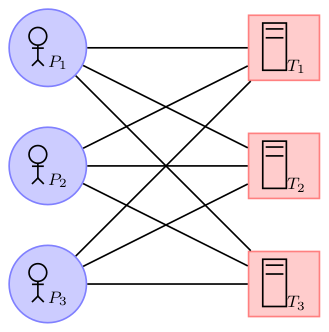
\includegraphics[width=0.85\linewidth]{figs/modeling-sums-tikz02.png}

\medskip
\modelhead{Sets}
\begin{itemize}
    \item \( I \) – Set of agents (or workers), indexed by \( i \).
    \item \( J \) – Set of tasks (or jobs), indexed by \( j \).
\end{itemize}

\medskip
\modelhead{Parameters}
\begin{itemize}
    \item \( c_{ij} \) – Cost associated with assigning agent \( i \in I\) to task \( j \in J\).
\end{itemize}

\medskip
\modelhead{Variables}
\begin{itemize}
    \item \( x_{ij} \) – Binary decision variable, where:
          \[
          x_{ij} =
          \begin{cases}
          1, & \text{if agent } i \text{ is assigned to task } j, \\
          0, & \text{otherwise}.
          \end{cases}
          \]
\end{itemize}

\medskip
\modelhead{Model}

\begin{align*}
\min \quad & \sum_{i \in I} \sum_{j \in J} c_{ij} x_{ij}   \tag{Total cost}\label{eq:assignment_objective} \\
\st        & \sum_{j \in J} x_{ij} = 1 &&\quad \text{for all } i \in I   \tag{Each agent one task}\label{eq:assignment_agent_constraint} \\
             & \sum_{i \in I} x_{ij} = 1 &&\quad \text{for all } j \in J   \tag{Each task one agent}\label{eq:assignment_task_constraint} \\
             & x_{ij} \in \{0,1\} &&\quad \text{for all } i \in I,\, j \in J.   \tag{Binary}\label{eq:assignment_binary_constraint}
\end{align*}

\medskip
\underline{\textbf{Explanation}}:
\begin{itemize}
    \item \textbf{Objective function} \eqref{eq:assignment_objective}: Minimizes the total assignment cost based on given costs \( C_{ij} \).
    \item \textbf{Constraints} \eqref{eq:assignment_agent_constraint}: Each agent is assigned to exactly one task.
    \item \textbf{Constraints} \eqref{eq:assignment_task_constraint}: Each task is assigned to exactly one agent.
    \item \textbf{Binary constraint} \eqref{eq:assignment_binary_constraint}: Ensures each assignment is either made (\( x_{ij} = 1 \)) or not (\( x_{ij} = 0 \)).
\end{itemize}

%This problem can be efficiently solved using algorithms such as the \textbf{Hungarian method} for the classical case or integer programming solvers like \textbf{branch and bound} for larger instances.

%The \emph{assignment problem} (machine/person to job/task assignment) seeks to assign tasks to machines in a way that is most efficient.   This problem can be thought of as having a set of machines that can complete various tasks (textile machines that can make t-shirts, pants, socks, etc) that require different amounts of time to complete each task, and given a demand, you need to decide how to alloacte your machines to tasks.
%
%Alternatively, you could be an employer with a set of jobs to complete and a list of employees to assign to these jobs.  Each employee has various abilities, and hence, can complete jobs in differing amounts of time.  And each employee's time might cost a different amout.  How should you assign your employees to jobs in order to minimize your total costs?

\begin{general}{Assignment Problem}{}{}
%Given $m$ machines and $n$ jobs, find a least cost assignment of jobs to machines. The cost of assigning job $j$ to machine $i$ is $c_{ij}$.
\end{general}
%

\begin{examplewithcode}{Machine Assignment}{\href{https://github.com/open-optimization/open-optimization-or-examples/blob/master/integer-programming/assignment-problem.ipynb}{Gurobipy}} 
A small manufacturing workshop has four specialized machines and four jobs to be completed today.  
Each machine can perform any job, but the time and energy cost vary depending on the job–machine combination.  
For example, Machine 0 might perform Job 2 very efficiently, while it would take much longer and cost more to complete Job 1.  
Management wants to assign exactly one job to each machine and exactly one machine to each job so that the \emph{total operating cost} is minimized.  
The cost matrix \(c_{ij}\) reflects the expected operating cost (in dollars) for assigning Machine \(i\) to Job \(j\).  

\modelhead{Sets}
\begin{itemize}
\item Let $I = \{0,1,2,3\}$ set of machines.
\item Let $J = \{0,1, 2,3\}$ be the set of tasks.
\end{itemize}

\modelhead{Parameters}
\begin{itemize}
\item $c_{ij}$ - the cost of assigning machine $i$ to job $j$.
\end{itemize}

\modelhead{Variables}
\begin{itemize}
\item Let
\begin{equation*}
x_{ij} = \begin{cases}
1 & \text{if machine $i$ assigned to job $j$}\\
0 & \text{otherwise.}
\end{cases}
\end{equation*}
\end{itemize}

\modelhead{Model}
\begin{align*}
\min \quad & \sum_{i \in I,\, j \in J} c_{ij} x_{ij}   \tag{Total cost} \\
\st        & \sum_{i \in I} x_{ij} = 1 &&\quad \text{for all } j \in J   \tag{Each job assigned one machine} \\
             & \sum_{j \in J} x_{ij} = 1 &&\quad \text{for all } i \in I   \tag{Each machine assigned one job} \\
             & x_{ij} \in \{0,1\} &&\quad \text{for all } i \in I,\, j \in J.
\end{align*}
\end{examplewithcode}

\begin{examplewithallcode}{School Bus Routing Problem}
{https://github.com/open-optimization/open-optimization-or-book/blob/master/Intro-Math-Programming/baseText/optimization/optimization-examples/school-bus-excel.xlsx}
{https://github.com/open-optimization/open-optimization-or-book/tree/master/Intro-Math-Programming/baseText/optimization/optimization-examples/school_bus_pulp.ipynb}
{https://github.com/open-optimization/open-optimization-or-book/tree/master/Intro-Math-Programming/baseText/optimization/optimization-examples/school_bus_gurobi.ipynb}

A school district has a set of schools \( I \) and a fleet of school buses \( J \). Each bus needs to be assigned to a school every morning to pick up students. The cost \( c_{ij} \) represents the fuel cost for bus \( j \) to reach school \( i \) and complete the route. The district aims to minimize the total fuel cost while ensuring that each school is served by exactly one bus and each bus is assigned to exactly one school.

The fuel costs can be found in the following table.  They are also in csv file format \href{https://github.com/open-optimization/open-optimization-or-examples/blob/master/integer-programming/school_bus_data.csv}{here}.
\begin{tabular}{l|ccccc}
\toprule
Bus/School & School A & School B & School C & School D & School E \\
\midrule
Bus 1 & 50 & 80 & 60 & 90 & 100 \\
Bus 2 & 60 & 85 & 55 & 70 & 110 \\
Bus 3 & 75 & 65 & 50 & 85 & 90 \\
Bus 4 & 70 & 90 & 55 & 80 & 95 \\
Bus 5 & 80 & 70 & 60 & 75 & 85 \\
\bottomrule
\end{tabular}

We can model this as follows:

\modelhead{Sets}
\begin{itemize}
    \item \(i \) - Index for schools, \(i \in I\)
    \item \(j \) - Index for buses, \(j \in J\)
\end{itemize}

\modelhead{Parameters}
\begin{itemize}
    \item \(c_{ij} \) - Fuel cost for bus \(j\) to serve school \(i\).
\end{itemize}

\modelhead{Variables}
\begin{itemize}
    \item \(x_{ij} \) - 1 if bus \(j\) is assigned to school \(i\), 0 otherwise.
\end{itemize}

\modelhead{Model}
\begin{align*}
\min \quad & \sum_{i \in I,\, j \in J} c_{ij} x_{ij}   \tag{Total fuel cost} \\
\st        & \sum_{i \in I} x_{ij} = 1 &&\quad \text{for all } j \in J   \tag{Each bus serves one school} \\
             & \sum_{j \in J} x_{ij} = 1 &&\quad \text{for all } i \in I   \tag{Each school served by one bus} \\
             & x_{ij} \in \{0,1\} &&\quad \text{for all } i \in I,\, j \in J.
\end{align*}
\end{examplewithallcode}

\begin{examplewithallcode}{Hiring for tasks}
{https://github.com/open-optimization/open-optimization-or-book/blob/master/Intro-Math-Programming/baseText/optimization/optimization-examples/assignment-problem-excel.xlsx}
{https://github.com/open-optimization/open-optimization-or-book/tree/master/Intro-Math-Programming/baseText/optimization/optimization-examples/assignment_problem_pulp.ipynb}
{https://github.com/open-optimization/open-optimization-or-book/tree/master/Intro-Math-Programming/baseText/optimization/optimization-examples/assignment_problem_gurobi.ipynb}
Recall Example~\ref{example:hiring-for-tasks}.  
We define the following sets, parameters, and variables to construct the mathematical model.

\modelhead{Sets}
\begin{itemize}
    \item $I = \{1, 2, 3\}$, the set of people.
    \item $J = \{1, 2, 3\}$, the set of tasks.
\end{itemize}

\modelhead{Parameters}
\begin{itemize}
    \item $C_{ij}$, the cost of assigning person $i \in I$ to task $j \in J$. The costs are given in the following table:\footnote{The numerical cost matrix used in this example is similar to one appearing in an introductory assignment-problem tutorial at \url{https://www.excel-easy.com/examples/assignment-problem.html}; if the values were taken from that source rather than independently chosen, this footnote serves as attribution.}
    \begin{align*}
        C = \begin{bmatrix}
            40 & 47 & 80 \\
            72 & 36 & 58 \\
            24 & 61 & 71 \\
        \end{bmatrix}
    \end{align*}
\end{itemize}

\modelhead{Variables}
\begin{itemize}
    \item $x_{ij} = 
    \begin{cases} 
    1 & \text{if person } i \text{ is assigned to task } j \\
    0 & \text{otherwise}
    \end{cases}$ for all $i \in I, j \in J$.
\end{itemize}

\modelhead{Model}

The complete model is:
\begin{align*}
\min \quad & \sum_{i \in I} \sum_{j \in J} C_{ij} x_{ij}   \tag{Total cost} \\
\st        & \sum_{j \in J} x_{ij} = 1 &&\quad \text{for all } i \in I   \tag{Each person one task} \\
             & \sum_{i \in I} x_{ij} = 1 &&\quad \text{for all } j \in J   \tag{Each task one person} \\
             & x_{ij} \in \{0,1\} &&\quad \text{for all } i \in I,\, j \in J.
\end{align*}

This model assigns each person to exactly one task and each task to exactly one person at minimum total cost.

\end{examplewithallcode}

The assignment problem has an integrality property, such that if we remove the binary restriction on the $x$ variables (now just non-negative, i.e., $x_{ij} \ge 0$) then we still get binary assignments, despite the fact that it is now an LP.  This property is very interesting and useful. 

Of course, the objective function might not quite what we want, we might be interested ensuring that the team with the worst assignment is as good as possible (a fairness criteria). One way of doing this is to modify the assignment problem using a max-min objective:

\medskip \textbf{Max-min Assignment-like Formulation} \\
\begin{eqnarray}
\max & z  \nonumber \\
%    s.t. & \sum_{i=1}^{n} x_{ij} = 1,~~  && \forall j = 1,\dots,n \nonumber \\
%         & \sum_{j=1}^{n} x_{ij} = 1,~~  && \forall i = 1,\dots,n \nonumber \\
%         & x_{ij} \ge 0,~~               && \forall i = 1,\dots,n, \; j = 1,\dots,n \nonumber \\
%         & z \le \sum_{i=1}^{n} C_{ij} x_{ij},~~ && \forall j = 1,\dots,n. \nonumber
\end{eqnarray}
%
%Does this formulation have the integrality property (it is not an assignment problem)?  Consider a very simple example where two teams are to be assigned to two projects and the teams give the projects the following rankings:
\begin{table}[h!] \begin{center} \begin{tabular} {|c||c|c|}
\hline           & Project~1 & Project~2 \\ \hline \hline
\hline Team 1    & 2  & 1  \\
\hline Team 2    & 2  & 1 \\ \hline
\end{tabular} \end{center} \end{table}
%Both teams prefer Project 2.  For both problems, if we remove the binary restriction on the
%$x$-variable, they can take values between (and including) zero and one. For the assignment problem the optimal solution will have $z=3$, and fractional $x$-values will not improve $z$. For the max-min assignment problem this is not the case, the optimal solution will have $z=1.5$, which occurs when each team is assigned half of each project (i.e., for Team 1 we have $x_{11} = 0.5$ and $x_{21} = 0.5$).
\medskip \textbf{Min-max Assignment-like Formulation} \\
\begin{align*}
\min \quad & z  \nonumber \\
\st        & z \geq \sum_{i \in I} C_{i j} x_{i j},~~ &&\quad \text{for all } j \in J \\
   & \sum_{i \in I} x_{i j} = 1,~~ &&\quad \text{for all } j \in J \\
         & \sum_{j \in J} x_{i j} = 1,~~ &&\quad \text{for all } i \in I \\
         & x_{i j} \ge 0,~~ &&\quad \text{for all } i \in I, \; j \in J
\end{align*}

\medskip \textbf{Does this formulation have the integrality property?}  
(It is not an assignment problem.)

Consider a simple example where two teams are to be assigned to two projects, and the teams provide the following rankings (lower ranking is better):

\begin{table}[h!] 
\begin{center} 
\begin{tabular} {|c||c|c|}
\hline           & Project~1 & Project~2 \\ \hline \hline
Team 1    & 2  & 1  \\
Team 2    & 2  & 1 \\ \hline
\end{tabular} 
\end{center} 
\end{table}

Both teams prefer Project 2.

If we remove the binary restriction on the \(x\)-variable, the values can range between 0 and 1.  
For the original assignment problem, the optimal solution has \(z=2\), and fractional \(x\)-values do not improve \(z\).  

For the min-max assignment problem, however, this is not the case. The optimal solution has \(z=1.5\), occurring when each team is assigned half of each project (i.e., for Team 1, we have \(x_{11} = 0.5\) and \(x_{21} = 0.5\)). By fractionalizing assignments, the worst-case project cost is minimized.

\begin{casestudybox}{Preference-Based Housing Assignment in Uruguayan Cooperatives}

Housing cooperatives in Uruguay play a crucial role in providing affordable housing to their members. Traditionally, once a new cooperative building was completed, the assignment of individual housing units was conducted through a random draw. This method, while simple, ignored individual preferences such as sunlight orientation, floor level, and proximity to shared facilities. Recognizing the potential for improved member satisfaction, researchers developed an alternative assignment method based on \textbf{mixed-integer programming (MIP)}.

\subsection*{The Challenge}
In Uruguayan housing cooperatives, every member is entitled to a housing unit. Since the assignment process happens only once per building, it is crucial to ensure fairness while maximizing overall satisfaction. The existing lottery-based system failed to account for members' preferences, sometimes leading to dissatisfaction and informal exchanges of units after the assignment. The challenge was to develop a new assignment process that:
\begin{itemize}
    \item Ensured fairness among all members,
    \item Incorporated individual preferences,
    \item Was easy to explain and implement,
    \item Could be executed in real time during cooperative meetings.
\end{itemize}

\subsection*{The Solution: A Two-Stage Optimization Model}
A team of researchers proposed a \textbf{two-stage mixed-integer programming (MIP) model} to address these concerns. The assignment problem was formulated with the following structure:

\textbf{Stage 1 – Ensuring Fairness:} The model maximizes the satisfaction of the least satisfied member. This ensures that no one is assigned an extremely undesirable unit.

\textbf{Stage 2 – Optimizing Global Satisfaction:} Given the fairness constraints from Stage 1, the model then seeks to optimize the total satisfaction across all cooperative members.

The assignment process was implemented using a software tool called \textbf{MTAV (Mejor Tecnología de Asignación de Viviendas – A Better Technology for Housing Assignment)}, designed to be transparent and user-friendly.

\subsection*{Implementation and Results}
The first real-world test of the model occurred in \textbf{2016} with the \textbf{Virazón housing cooperative}, consisting of \textbf{50 members}. Before deployment, the cooperative members reviewed and voted to approve the new method. Their individual housing preferences were collected and input into the system.

On the day of the assignment:
\begin{itemize}
    \item The housing allocation was carried out in \textbf{real-time} during a cooperative meeting.
    \item The results were projected on a large screen for transparency.
    \item A notary was present to certify the fairness of the process.
    \item The optimization model took only a few \textbf{seconds} to compute the assignments.
\end{itemize}

The outcomes were striking:
\begin{itemize}
    \item \textbf{Four-bedroom apartments:} Both members received their first-choice units.
    \item \textbf{Three-bedroom apartments:} More than 37\% of members received their first-choice unit, and the average satisfaction ranking was significantly better than a random assignment.
    \item \textbf{Two-bedroom apartments:} Over \textbf{half} of the members received one of their top four choices, with all assignments being significantly better than expected under a random draw.
\end{itemize}

The cooperative members overwhelmingly supported the new system, reporting higher satisfaction compared to previous assignment methods.

\subsection*{Broader Impact}
Since the successful implementation at Virazón, \textbf{over 30 housing cooperatives} in Uruguay have adopted the model. Further developments have included:
\begin{itemize}
    \item The introduction of a \textbf{graphical user interface} to make data input more intuitive.
    \item Support for \textbf{partial order preferences}, allowing members to indicate that they have no strong preference between certain units.
    \item Exploration of additional fairness criteria and trade-offs between individual and collective satisfaction.
\end{itemize}

Beyond its technical achievements, this case study highlights how \textbf{operations research techniques} can be applied to solve real-world social challenges. By integrating mathematical optimization with participatory decision-making, the project has significantly improved the way housing is assigned in cooperative communities, setting a precedent for future applications in housing policy and beyond.

\subsection*{Optimization models}

The optimization model required the following input parameters and variables:

\modelhead{Sets}
\begin{itemize}
    \item $I$: Set of cooperative members needing housing assignments.
    \item $J$: Set of available housing units.
\end{itemize}

\modelhead{Parameters}
\begin{itemize}
    \item $p_{ij}$: Preference score of member $i$ for housing unit $j$, where lower values indicate higher preference (e.g., $1$ = most preferred).
    \item Some versions of the model supported \textbf{partial order preferences}, allowing members to express equal preference for multiple units.
\end{itemize}

\modelhead{Variables}
\begin{itemize}
    \item $x_{ij} \in \{0,1\}$: Binary variable indicating whether member $i$ is assigned to unit $j$:
    \[
    x_{ij} =
    \begin{cases} 
        1, & \text{if member } i \text{ is assigned to unit } j \\ 
        0, & \text{otherwise} 
    \end{cases}
    \]
\end{itemize}

\subsection*{Two-Stage Optimization Approach}

\textbf{Stage 1: Ensuring Fairness}

\begin{itemize}
    \item Define $S$ as the satisfaction level of the least satisfied member:
    \[ S = \min_{i \in I} \sum_{j \in J} p_{ij} x_{ij} \]
    \item Ensure each member is assigned exactly one unit and each unit is assigned to exactly one member.
\end{itemize}
This is achieved by the model
\begin{align*}
    S = \min \; & z \\
\st        & z \geq \sum_{j \in J} p_{i j} x_{i j} &&\quad \text{for all } i \in I \\
                 & \sum_{j \in J} x_{i j} = 1 &&\quad \text{for all } i \in I \\
                 & \sum_{i \in I} x_{i j} = 1 &&\quad \text{for all } j \in J \\
                 & x_{i j} \in \{0,1\} &&\quad \text{for all } i \in I, \; j \in J \\
                 & z \in \mathbb{R}
\end{align*}

\textbf{Stage 2: Optimizing Global Satisfaction}

\begin{itemize}
    \item Given the fairness threshold $S$ from Stage 1, optimize total satisfaction:
    \[ \min \sum_{i \in I} \sum_{j \in J} p_{ij} x_{ij} \]
    \item Subject to the fairness constraint:
    \[ \sum_{j \in J} p_{ij} x_{ij} \leq S, \quad \forall i \in I \]
    \item Ensures that no member receives a unit less desirable than the worst outcome allowed by Stage 1.
\end{itemize}
This is achieved by the model
\begin{align*}
\min \quad & \sum_{i \in I} \sum_{j \in J} p_{i j} x_{i j} \\
\st        & \sum_{j \in J} x_{i j} = 1 &&\quad \text{for all } i \in I \\
                 & \sum_{i \in I} x_{i j} = 1 &&\quad \text{for all } j \in J \\
                 & \sum_{j \in J} p_{i j} x_{i j} \leq S &&\quad \text{for all } i \in I \\
                 & x_{i j} \in \{0,1\} &&\quad \text{for all } i \in I, \; j \in J
\end{align*}

\subsection*{Implementation Notes}

\begin{itemize}
    \item The model was formulated as a \textbf{mixed-integer programming (MIP)} model.
    \item The assignment was computed in \textbf{real-time} during cooperative meetings.
    \item The \textbf{MTAV} software was used to collect user preferences and compute assignments efficiently.
    \item The system ensured transparency, allowing cooperative members to verify their preferences before the final optimization.
\end{itemize}

\subsection*{References}
\begin{itemize}
\item \href{https://ifors.org/newsletter/ifors-news-dec-2024.pdf}{IFORS Newsletter December 2024 -  Section 4: OR Impact}
\item  M. Prino, E. Sánchez, H. Cancela. “Optimal distribution of habitational units in a cooperative: A mathematical application to optimize satisfaction” (text in Spanish). Proceedings of CLEI 2016 (Conferencia Latinoamericana de Informática), 2016. \url{https://doi.org/10.1109/CLEI.2016.7833357}
\end{itemize}

\end{casestudybox}

\section{Modeling Tricks}

\subsection{Maximizing a minimum}
When the constraints could be general, we will write $x \in X$ to define general constraints.  For instance, we could have $X = \{ x \in \R^n : Ax \leq b\}$ of $X  = \{ x \in \R^n : Ax \leq b, x \in \Z^n\}$ or many other possibilities.  

Consider the problem 

\begin{align*}
\max   \quad & \min \{x_1, \dots, x_n\}\\
\text{ such that } \quad &  x \in X
\end{align*}
Having the minimum on the inside is inconvenient.  To remove this, we just define a new variable $y$ and enforce that $y \leq x_i$ and then we maximize $y$.  Since we are maximizing $y$, it will take the value of the smallest $x_i$.  Thus, we can recast the problem as

\begin{align*}
\max\quad    & y\\
\text{ such that } \quad  & y \leq x_i \ \text{ for }\  i=1, \dots, n \\
&  x \in X
\end{align*}

\begin{examplewithallcode}{Minimizing an Absolute Value}
{}
{https://github.com/open-optimization/open-optimization-or-book/tree/master/Intro-Math-Programming/baseText/optimization/optimization-examples/absolute_value_pulp.ipynb}
{https://github.com/open-optimization/open-optimization-or-book/tree/master/Intro-Math-Programming/baseText/optimization/optimization-examples/absolute_value_gurobi.ipynb}
Note that
$$
|t| = \max(t, -t),
$$
so to minimize $|t|$ we can instead write

\begin{align*}
\min \quad & z\\
\st        & t \leq z\\
           & -t \leq z.
\end{align*}

The accompanying code applies this trick to find the point minimizing the total
absolute distance to several given points (whose optimum is their median).
\end{examplewithallcode}

